% Schematic redraw of the source figure; not to scale.
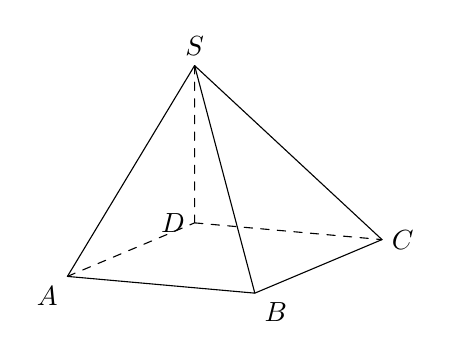
\begin{tikzpicture}[line cap=round,line join=round,scale=0.85]
  \coordinate (A) at (-2.4,0);
  \coordinate (B) at (0.4,-0.25);
  \coordinate (C) at (2.3,0.55);
  \coordinate (D) at (-0.5,0.8);
  \coordinate (S) at (-0.5,3.15);

  % Hidden back edges and the perpendicular altitude SD.
  \draw[dashed] (A)--(D) (D)--(C) (S)--(D);
  % Visible base edges and lateral edges.
  \draw (A)--(B)--(C);
  \draw (S)--(A) (S)--(B) (S)--(C);

  \node[below left] at (A) {$A$};
  \node[below right] at (B) {$B$};
  \node[right] at (C) {$C$};
  \node[left] at (D) {$D$};
  \node[above] at (S) {$S$};
\end{tikzpicture}
